\documentclass[fleqn,11pt]{ExcelAtFIT} % Document font size and equations flushed left


%--------------------------------------------------------
%--------------------------------------------------------
%	REVIEW vs. FINAL VERSION
%--------------------------------------------------------

%   LEAVE this line commented out for the REVIEW VERSIONS
%   UNCOMMENT this line to get the FINAL VERSION
%\ExcelFinalCopy


%--------------------------------------------------------
%--------------------------------------------------------
%	LANGUAGE
%--------------------------------------------------------
%   Recommended language for Excel@FIT paper is English.
%   However, in emergency, you can write in Czech or Slovak.
%   In such a case, uncomment one of these lines to localize the template.
%--------------------------------------------------------
%\ExcelSlovakLabels
%\ExcelCzechLabels


%--------------------------------------------------------
%--------------------------------------------------------
%	PDF CUSTOMIZATION
%--------------------------------------------------------

\hypersetup{
	pdftitle={Verification of Pointer Programs Based on Forest Automata},
	pdfauthor={Martin Hruška},
	pdfkeywords={Forest Automata, Formal Verification, Static Analysis, Complex Data Structures, Tree Automata, Backward Run, Predicate Abstraction}
}

\usepackage{comment}
\usepackage{tikz}
\usepackage{subcaption}
\usetikzlibrary{calc,matrix,backgrounds,fit,shapes,arrows}

\newcommand{\vata}[0]{the VATA library}
\newcommand{\Vata}[0]{The VATA library}
\newcommand{\fagr}[0]{\otimes t_1, \ldots, t_n}
\newcommand{\funcdecl}[3]{#1: #2 \rightarrow #3}
\newcommand{\subst}[2]{[#1/#2]} %co, za co
\newcommand{\bexmp}[0]{\noindent\rule{\textwidth}{0.4pt} \begin{example}}
\newcommand{\eexmp}[0]{\end{example} \noindent\rule{\textwidth}{0.4pt}}
\newcommand{\symset}[0]{\mathbb{S}}
\newcommand{\instrset}[0]{\mathbb{I}}
\newcommand{\regs}[0]{\mathbb{G}}
\newcommand{\regsset}[0]{\{r_1, \ldots, r_m\}}
\newcommand{\regssub}[2]{\regs [#1 := #2]}
\newcommand{\regssubmin}[3]{\regs \setminus \{#3\} [#1 := #2]}
\newcommand{\symstate}[3]{(#1, #2, #3)}
\newcommand{\stdsym}[0]{\symstate{F}{\regs}{I}}
\newcommand{\natnum}[0]{\mathbb{N}}

\newcommand{\lfunc}[2]{\lambda #1 \,:\, #2}
\newcommand{\lfuncp}[3]{(\lambda #1 \,:\, #2)(#3)}

\newcommand{\ddispl}[0]{Displ}
\newcommand{\droot}[0]{Root}
\newcommand{\rref}[0]{RR=(\droot,\ddispl)}
\newcommand{\rreftuple}[2]{(#1,#2)}
\newcommand{\rrefreg}[1]{#1=(\droot,\ddispl)}
\newcommand{\ddata}[0]{D = (T,S,V,MB)}

\newcommand{\grev}[0]{g}
\newcommand{\grevinter}[0]{\symset \times \instrset \rightarrow \symset}

\newcommand{\code}[1]{\small{\texttt{#1}}}
\newcommand{\codix}[1]{\emph{\code{#1}}}

\newcommand{\sbwd}[0]{S^{B}_{i}}
\newcommand{\isfwd}[0]{I^{F}}
\newcommand{\sfwd}[0]{S^{F}_{i}}
\newcommand{\ftraceseq}[0]{S^{F}_n \cdots S^{F}_1}
\newcommand{\ftrace}[0]{FT}

\newcommand{\btraceseq}[0]{S^{B}_1 \cdots S^{B}_n}
\newcommand{\btrace}[0]{BT}
\newcommand{\isbwd}[0]{I^{B}}
\newcommand{\bstdsym}[0]{\symstate{F}{\regs}{\isbwd}}


%--------------------------------------------------------
%--------------------------------------------------------
%	ARTICLE INFORMATION
%--------------------------------------------------------

\ExcelYear{2015}

\PaperTitle{Verification of Pointer Programs Based on Forest Automata}

\Authors{Martin Hruška*}
\affiliation{*%
  \href{mailto:xhrusk16@stud.fit.vutbr.cz}{xhrusk16@stud.fit.vutbr.cz},
  \textit{Faculty of Information Technology, Brno University of Technology}}
%%%%--------------------------------------------------------
%%%% in case there are multiple authors, use the following fragment instead
%%%%--------------------------------------------------------
%\Authors{Jindřich Novák*, Janča Dvořáková**}
%\affiliation{*%
%  \href{mailto:xnovak00@stud.fit.vutbr.cz}{xnovak00@stud.fit.vutbr.cz},
%  \textit{Faculty of Information Technology, Brno University of Technology}}
%\affiliation{**%
%  \href{mailto:xdvora00@stud.fit.vutbr.cz}{xdvora00@stud.fit.vutbr.cz},
%  \textit{Faculty of Information Technology, Brno University of Technology}}

\Keywords{Forest Automata --- Formal Verification --- Static Analysis --- Complex Data Structures --- Tree Automata --- Backward Run --- Predicate Abstraction}

%\Supplementary{\href{http://youtu.be/S3msCdn3fNM}{Demonstration Video} --- \href{http://excel.fit.vutbr.cz/}{Downloadable Code}}


%--------------------------------------------------------
%--------------------------------------------------------
%	ABSTRACT and TEASER
%--------------------------------------------------------

\Abstract{
  Forest automata are one of the formalisms recently used for analysis and verification of programs manipulating dynamic data structures.
  In the area of shape analysis there exists a tool Forester employing forest automata.
  Forest automata are based on tree automata and Forester has its own implementation of tree automata.
  However, there is the VATA library which implements the~efficient algorithms for the~tree automata manipulation,
  especially the efficient algorithms for the~checking inclusion of languages of tree automata what is an operation
  crucial also for the~verification procedure based on forest automata.
  The first goal of this work is to implement a version of Forester tool that uses the VATA library for tree automata manipulation.
  The second goal of this work is to extend forest automata based verification with backward run that checks whether
  a found error is a~spurious or a real one what could be used for refinement of predicate abstraction.
  The first goal has been already fulfilled and the variant of Forester using the VATA library successfully participated in the competition SV-COMP 2015.
  The part of the second goal is done only partially -- the backward run is already finished and predicate abstraction implementation is
  in progress.
}

%\Teaser{
%	\TeaserImage{placeholder.pdf}
%	\TeaserImage{placeholder.pdf}
%	\TeaserImage{placeholder.pdf}
%}



%--------------------------------------------------------
%--------------------------------------------------------
%--------------------------------------------------------
%--------------------------------------------------------
\begin{document}

\startdocument


%--------------------------------------------------------
%--------------------------------------------------------
%	ARTICLE CONTENTS
%--------------------------------------------------------

%--------------------------------------------------------
%--------------------------------------------------------
%--------------------------------------------------------
%--------------------------------------------------------
\section{Introduction}

The importance of computers in our everyday life has largely increased over the past few decades.
A~lot of us can only hardly imagine doing their jobs without help of an appropriate computer program
and we also spend a plenty of time using computers (e.g. personal computers or mobile devices) in leisure time.
The~computer programs are also often used in very critical instances like autopilot in an airplane.
But the growing number of applications of computer programs brings also the~need for their greater safety and security.

However, a guarantee of software safety and correctness is not an easy task
because the programs often go through many states during the computation
and it could be very time and space consuming or even impossible to check whether no undesirable behavior
happens in any of those states.
One of the approaches to ensure the software quality is \emph{testing} (and dynamic analysis) which is basically based
on running a program in the different contexts and with the different inputs
and matching a program behavior and the outputs with the expected ones.
This method can satisfy many of the requirements for the software quality and often cover the great space of the program behaviors
but on the~other side it is only possible to prove presence of the~errors using testing not their absence \cite{dijkstra}.
Moreover finding some errors during testing does not mean that all errors are eliminated.

The mentioned weakness of testing can be resolved by \emph{formal verification}
which is another approach to checking the program correctness.
Formal verification is the method for checking whether a given system meets a given specification \cite{fav:lecture}.
There are three main branches of formal verification.
The first one is \emph{model checking} which systematically explores the states of a~model (e.g. model of a program) to
prove that a~property holds along the whole model.
The second one is \emph{static analysis} which is done over a source code (or some modification of it) of a system
without its explicit execution.
One of the important and very widely used approaches in static analysis is called \emph{abstract interpretation} where the analysis is performed by
applying abstract transformers corresponding to the original program semantics over an abstract domain.
The last approach is \emph{theorem proving}.
It proves the program in a standard mathematical way -- starting from axioms and proving theorems to
verify the properties of a given system.
Theorem proving could be partially automated.

This work deals with a specific part of static analysis called \emph{shape analysis} which is focused on the verification of the programs manipulating
complex data structures (like the different kinds of lists and trees), typically allocated on the heap.
The properties checked for this class of programs are for example checking whether no dangling
pointers are dereferenced (no invalid dereferences), whether all allocated memory on a heap is also freed
during the program execution (no memory leaks) or whether there is not freed pointer without assigned memory (no invalid free).
There are different approaches to this kind of static analysis with the different advantages.
For example, the approach based on \emph{separation logic} \cite{seplog,seplog07} provides great scalability of a verification procedure.
On the other side, the automata based approach, particularly \emph{abstract regular tree model checking} (ARTMC) \cite{artmc}, is
superior in its flexibility and generality.
However, this work is focused on a verification procedure based on a concept of forest automata (FA) which
combines benefits of the both mentioned approaches.

Forest automata (FA) has been introduced in \cite{forester11,forester12} and they are an extension of finite automata or more precisely extension of finite tree automata (TA).
They are used as an abstract domain in related verification procedure over which a symbolic execution of an analyzed program is performed.
A~prototype of this verification procedure has been implemented in a tool called \emph{Forester}.
Forester verifies programs written in C~language and it can detect safety violations like invalid dereferences, invalid frees, memory leaks and also reachability of an error label.
It is yet able to verify non-trivial data structures like skip-lists of the second and the third level
but there is still a room for its improvement.
E.g., Forester currently does not support the complete C language syntax and %TODO
it is not also yet possible to check whether a found error is real or spurious.
It is also needed to refactor some parts of Forester code before any extension of the tool.
A~general goal of this work is to improve Forester in the areas described further.

Since FA are highly related to the finite tree automata the first goal of this work is to change
the underlying implementation of finite tree automata in Forester to \vata\ -- a state-of-the-art library for TA manipulation \cite{libvata}.
Particularly, this consists creating an interface between Forester and VATA to employ VATA as a TA library for Forester backend
which should bring better maintainability and modularity than having a special TA library implementation within Forester as it is now.
The second goal of this work is to design and implement \emph{backward run} for FA based verification
which enables checking spuriousness of an error found in a program.
The error could be spurious because too strong abstraction over FA is used.
The information gained by backward run could be used for the refinement of \emph{predicate abstraction} (one kind of abstraction over FA)
to prevent verification procedure from getting the same spurious error again.
This way of gradual refinement is based on \emph{counterexample-guided abstraction refinement} (CEGAR) \cite{cegar}.
However, Forester does not currently use the mentioned predicate abstraction but \emph{height abstraction} %TODO
because predicate abstraction needs backward run to be fully functional.
Height abstraction is less precise and less flexible compared to predicate abstraction so implementing predicate abstraction
enables analysis of even more complex data structures like red-black trees.
A~part of the second goal is an implementation of predicate abstraction using backward run in Forester.

This paper is structured as follows.
In Section \ref{sec:overview} a high level overview of shape analysis based on forest automata
is given.
Then the closer description of backward run and predicate abstraction takes a place in Section \ref{sec:br}.
Section \ref{sec:forvata} provides description of modification of Forester to use the VATA library as a backend.
Finally, conclusions of the work is given in Section \ref{sec:concl}.

%--------------------------------------------------------
%--------------------------------------------------------
%--------------------------------------------------------
%--------------------------------------------------------
\section{Overview of Verification Method}
\label{sec:overview}

\begingroup
\tikzset{every picture/.style={scale=1}}%
\begin{figure*}[t]
	\centering
	\begin{subfigure}{0.5\textwidth}
	\centering
		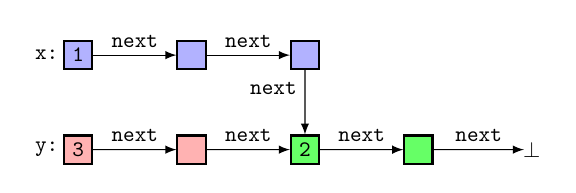
\begin{tikzpicture}[
  scale=0.8,
  transform shape,
]

  \tikzstyle{memnode}=[draw,rectangle,fill=lightgray,thick,minimum height=4.5mm, minimum width=4.5mm,inner sep=1mm,node distance=18mm,font=\tt]
  \tikzstyle{memnodeblue}=[draw,rectangle,fill=blue!30,thick,minimum height=4.5mm, minimum width=4.5mm,inner sep=1mm,node distance=18mm,font=\tt]
  \tikzstyle{memnodepink}=[draw,rectangle,fill=red!30,thick,minimum height=4.5mm, minimum width=4.5mm,inner sep=1mm,node distance=18mm,font=\tt]
  \tikzstyle{memnodegreen}=[draw,rectangle,fill=green!60,thick,minimum height=4.5mm, minimum width=4.5mm,inner sep=1mm,node distance=18mm,font=\tt]

  \tikzstyle{nullnode}=[node distance=18mm,label=center:$\bot$]
  \tikzstyle{varnode}=[font=\tt]
  \tikzstyle{refnode}=[fill=green!20,minimum height=4.5mm, minimum width=4.5mm,inner sep=1mm,font=\tt]

  \tikzstyle{pointer}=[draw,->,>=latex]
  \tikzstyle{ptrlab}=[above,font=\tt]

  % nodes
  \node[memnodeblue] (x1) at (0mm,0mm) {1};
  \node[memnodeblue] (x2) [right of=x1] {};
  \node[memnodeblue] (x3) [right of=x2] {};

  \node[memnodepink] (y1) [below of=x1, yshift=3mm] {3};
  \node[memnodepink] (y2) [right of=y1] {};

  \node[memnodegreen] (join) [right of=y2] {2};
  \node[memnodegreen] (j2) [right of=join] {};
  \node[nullnode] (j2null) [right of=j2] {};

  \node[varnode,node distance=5mm] (x) [left of=x1] {x:};
  \node[varnode,node distance=5mm] (x) [left of=y1] {y:};

  % pointers
  \draw[pointer] (x1)    -- node[ptrlab]   {next} (x2);
  \draw[pointer] (x2)    -- node[ptrlab]   {next} (x3);
  
  \draw[pointer] (x3)    -- node[ptrlab,xshift=-5mm]   {next} (join);

  \draw[pointer] (y1)    -- node[ptrlab]   {next} (y2);
  \draw[pointer] (y2)    -- node[ptrlab]   {next} (join);

  \draw[pointer] (join)  -- node[ptrlab]  {next}     (j2);
  \draw[pointer] (j2)    -- node[ptrlab]  {next}     (j2null);

\end{tikzpicture}

		\vspace{0.55cm}
		\caption{A~heap graph}
		\label{subfig:graph}
	\end{subfigure}%
	~
	\hspace{0.5cm}
	\begin{subfigure}{0.5\textwidth}
	\centering
		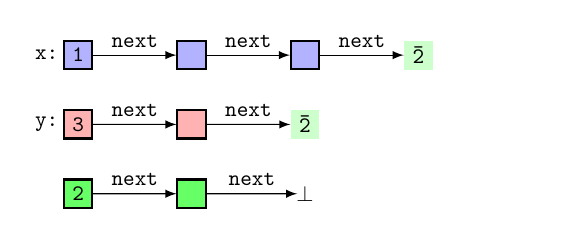
\begin{tikzpicture}[
  scale=0.8,
  transform shape,
  node distance=18mm
]

  \tikzstyle{memnode}=[draw,rectangle,fill=lightgray,thick,minimum height=4.5mm, minimum width=4.5mm,inner sep=1mm,node distance=18mm,font=\tt]
  \tikzstyle{memnodeblue}=[draw,rectangle,fill=blue!30,thick,minimum height=4.5mm, minimum width=4.5mm,inner sep=1mm,node distance=18mm,font=\tt]
  \tikzstyle{memnodepink}=[draw,rectangle,fill=red!30,thick,minimum height=4.5mm, minimum width=4.5mm,inner sep=1mm,node distance=18mm,font=\tt]
  \tikzstyle{memnodegreen}=[draw,rectangle,fill=green!60,thick,minimum height=4.5mm, minimum width=4.5mm,inner sep=1mm,node distance=18mm,font=\tt]

  \tikzstyle{nullnode}=[node distance=18mm,label=center:$\bot$]
  \tikzstyle{varnode}=[font=\tt]
  \tikzstyle{refnode}=[fill=green!20,minimum height=4.5mm, minimum width=4.5mm,inner sep=1mm,font=\tt]

  \tikzstyle{pointer}=[draw,->,>=latex]
  \tikzstyle{ptrlab}=[above,font=\tt]

  % nodes
  \node[memnodeblue] (x1)  at (0mm,0mm) {1};
  \node[memnodeblue] (x2) [right of=x1] {};
  \node[memnodeblue] (x3) [right of=x2] {};

  \node[memnodepink] (y1) [below of=x1, yshift=7mm] {3};
  \node[memnodepink] (y2) [right of=y1] {};

  \node[refnode] (joinsbst1) [right of=x3] {\=2};
  \node[refnode] (joinsbst2) [right of=y2] {\=2};

  \node[memnodegreen] (join) [below of=y1, yshift=7mm] {2};
  \node[memnodegreen] (j2) [right of=join] {};
  \node[nullnode] (j2null) [right of=j2] {};

  \node[varnode,node distance=5mm] (x) [left of=x1] {x:};
  \node[varnode,node distance=5mm] (x) [left of=y1] {y:};
  
  \node (placeholder) [right of=joinsbst1] {};
  

  % pointers
  \draw[pointer] (x1)    -- node[ptrlab]   {next} (x2);
  \draw[pointer] (x2)    -- node[ptrlab]   {next} (x3);
  \draw[pointer] (x3)    -- node[ptrlab]   {next} (joinsbst1);

  \draw[pointer] (y1)    -- node[ptrlab]   {next} (y2);
  \draw[pointer] (y2)    -- node[ptrlab]   {next} (joinsbst2);

  \draw[pointer] (join)  -- node[ptrlab]   {next} (j2);
  \draw[pointer] (j2)    -- node[ptrlab]   {next} (j2null);

\end{tikzpicture}

		\caption{A~tree decomposition of the heap graph}
		\label{subfig:trees}
	\end{subfigure}%
	\vspace{0.5cm}
	\caption{
	Figure shows tree decomposition of a heap graph.
	The heap graph representing singly-linked list is shown in Figure \ref{subfig:graph}.
	The nodes could be labeled by a pointer variable that references allocated memory cell
	corresponding to the node.
	Moreover the~cut-points are labeled by an order number that they have in an ordering over
	the cut-points.
	In this case there are three cut-points with an order number $1$, $2$ and $3$.
	The graph is split to the three trees shown in Figure \ref{subfig:trees} by the heap decomposition.
	The~new trees could contain the references to another trees, in this case tree $1$ and tree $3$
	have the nodes referencing tree $2$.}
	\label{fig:graph}
\end{figure*}
\endgroup

This section provides a high level overview of the verification procedure based
on forest automata.
As it was already mentioned we consider only C programs manipulating dynamic data structures.
The simple examples of such structures are singly-linked lists or binary trees.
Consider a singly-linked list containing an (integer) data member and a pointer
to the next item in the list and also
consider two variables $x,y$ pointing the singly-linked list.
An instance of the singly-linked list allocated on a heap can be viewed as an oriented graph.
The nodes of the graph correspond to the allocated memory cells
and the edges of the graph are related to the pointers referencing
another allocated memory cell of the list.
Each node can be labeled by a name of the pointer variables that
reference the given node or it could be labeled by a data contained in the node.
The example of such a graph is shown in~Figure~\ref{fig:graph}.
We omit the data nodes in Figure \ref{fig:graph} for sake of clarity.
The figure shows that the variables $x$, $y$ points two singly-linked list (the blue and the red nodes) that
have common part (the green nodes).
The original heap graph is shown in Figure~\ref{subfig:graph}.
The tree decomposition, which is described later, is in Figure~\ref{subfig:trees}.

We can decompose the graph to a set of trees by the following method \cite{forester11}.
First we identify so called \emph{cut-points} \,---\, the nodes referenced by
one or more pointer variables or the nodes having more than one incoming edges.
The cut-points are then numbered by a depth-first traversal of the graph starting from
the nodes referenced by the pointer variables.
Indeed, the traversal and the numbering defines an ordering over the cut-points.
The graph at Figure \ref{fig:graph} has the three cut-points that are labeled by the numbers $1$,
$2$ and $3$ what denotes the node order in the cut-points ordering.
Then the graph is split to the trees with cut-point as the roots.
The new trees do not contain any cut-points.
The~graph at Figure~\ref{subfig:graph} is decomposed to the three trees that are shown at the bottom of the figure.
Finally, we redirect the edges leading to the nodes marked as the cut-points to the new nodes because the cut-points are now roots of the trees.
The new nodes replacing the cut-points are labeled by a number referencing to the tree that has a related cut-point like a root.
The example at Figure~\ref{subfig:trees} shows that tree $1$ and tree $3$ contains the nodes with the label $\overline{2}$
referencing tree~$2$.

The tuple of trees (created by graph decomposition) is called forest.
Such a forest could be accepted by a forest automaton as a member of its language.
A~forest automaton is a tuple of finite tree automata which are automata accepting trees instead of words (in comparison with finite automata).
The tree automata within a forest automaton are interconnected by references (that are also symbols in their alphabet).
Each of the tree automata accepts a set of trees and so we get a language of a forest
automaton by their Cartesian product what is a set of tuples of trees (connected by the mentioned references).
These tuples of trees then represents a state of a heap. %TODO speak about forests

%So far we have described how to represent dynamic data structures by forest automata.
Forest automata can be viewed also as an abstract domain in context of abstract interpretation
whereas a concrete domain is a set of heaps with allocated data structures \cite{atva13}.
It is also possible to define abstract transformers corresponding to the (concrete) program operations over forest automata.
The verification procedure is then performed as a symbolic execution
where the abstract transformers are gradually applied to abstract domain.
When an error like an invalid memory reference or invalid free is detected during the symbolic
execution it implies that it is possible that there is an error in the~program (but the error could be also spurious because
the forest automata overapproximate a state space of the original program).

It is possible to represent a dynamic data structure with bounded number of cut-points by the mentioned approach.
But it cannot be used for data structures with an unbounded number of cut-points like doubly-linked lists.
The unboudness comes from the fact that each node of a doubly-linked list is a a cut-point because
it is pointed by the next and also the previous member of the list.
This problem can be solved by introducing so-called \emph{boxes} \cite{forester13}.
Boxes are symbols hiding the repeating sub-graphs causing unboudness.
Then these sub-graphs are replaced by an hyperedge labeled by an appropriate box
and so a new hierarchical hypergraph with bounded number of cut-points is created.
More precisely, boxes can be viewed as forest automata representing the repeating subgraphs.
So it is still possible to represent the hypergraph with forest automata where
boxes are symbols of forest automata.
We get hierarchical forest automata this way because forest automata of lower level
are included as symbols in alphabets of forest automata of higher level.
Note that a forest automaton of certain level can contain in its alphabet only automata of lower level than its own level.

More technical details about a heap decomposition and forest automata could be found in \cite{forester11, forester13}.

\section{Backward Run and Predicate Abstraction}
\label{sec:br}

\begin{figure}[t]
	\centering
	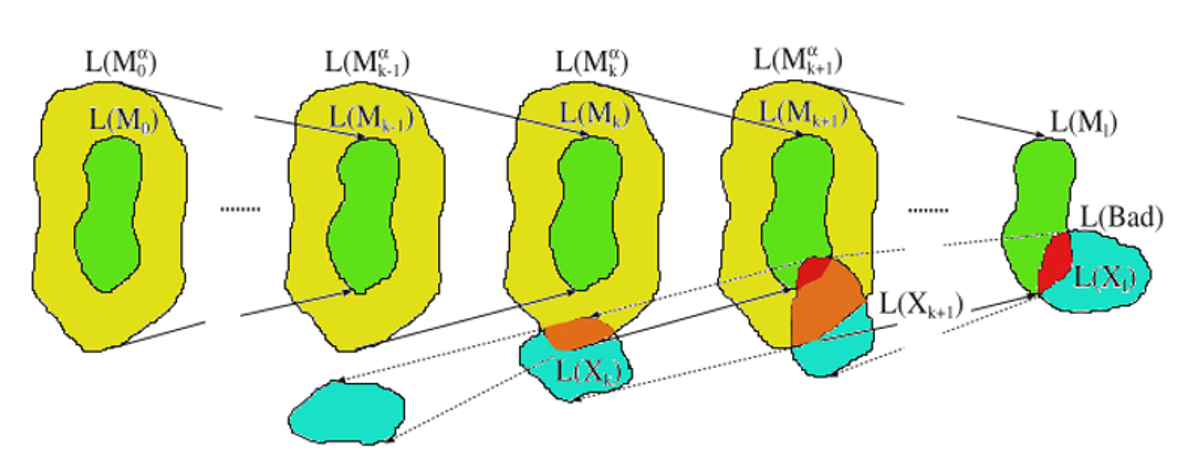
\includegraphics[width=1\linewidth]{artmc.png}
	\caption{
		Figure is taken from \cite{artmc}.
		Figure shows a forest automaton language $L(M_k)$ before (green area)
		and language $L(M_k^{\alpha})$ after (yellow area) abstraction where
		$k$ is the order of the state within symbolic execution.
		One oval consisting green and yellow part represents
		language of a forest automaton in a symbolic state of symbolic execution.
		Figure also shows how a forest automaton (and it language) is gradually changed
		by abstract transformers during a symbolic execution what is illustrated by the lines connecting ovals.
		A~found error is shown as a red area in the last oval.
		The backward run starts from this error and it finds
		that an error is spurious because an intersection (the orange areas) of forest automata language from backward (the blue ovals)
		and forward (the green and yellow areas) run is empty at the level of the symbolic state with the language $L(M^{\alpha}_{k-1})$.}
	\label{fig:bwrun}
\end{figure}

We have already covered how to represent dynamic data structures by forest automata in the previous section.
Forest automata are able to handle also infinite state spaces
rising from a possible unboudness of the mentioned dynamic data structures.
However, there is still the problem of state explosion that often makes
nearly impossible to finish verification procedure of a system in real time
and moreover, not even termination of the verification procedure is guaranteed at all.
Therefore the abstraction over the forest automata is introduced to increase probability of termination
and to accelerate the method.
The abstraction speeds up the computation by merging more states
of forest automata to one abstract state.
This also causes the overapproximation of the set of reachable
states of an analyzed system.
It can lead to reaching the error states in
an abstracted state space which are not present in the real system (the real system is a computer program in this case).
We can prevent reaching such spurious counterexamples by a refinement of the~abstraction
what avoids repeating of the abstraction of the states that lead to these errors.
The application of an abstraction over forest (and tree) automata in this work is based on \emph{abstract regular tree model checking} \cite{artmc}
and the refinement of the abstraction is based on \emph{counterexample-guided abstraction refinement} \cite{cegar}
as it was mentioned in the introduction section.

Forester now implements so called height abstraction.
This abstraction merges states whose languages (note that a language of state is a set of trees) are equal
when the trees of the languages are compared only to the given depth.
The main problem of this abstraction technique is the low ability of refinement.
The only way of refinement is by the parameter defining the depth of tree comparison
what does not ensure that a found spurious error will not be found again.
The~abstraction allowing more fine tuning is so called \emph{predicate abstraction} \cite{artmc}
that introduces a set of predicates and merges the states in which the same predicates hold.
When a spurious counterexample is found, then the set of predicates is extended by
a predicate that prevents reaching the spurious counterexample again
and the~verification procedure is rerun with the new predicate.

Finding the new predicate and checking spuriousness of an error is done by \emph{backward run}.
A~backward run starts from the forest automata modelling a~heap with a found error and
reverting gradually each abstract operation over the forest automata
in~backward order to the (forward) symbolic execution.
When an automata with an empty language is get by a reverse abstract transformation then the error is spurious.
The~last automaton of backward run with a non empty language is then used as a new predicate.
Backward run is illustrated by Figure \ref{fig:bwrun} and the illustration
is further described in the caption of the figure.

An operation often needed during backward run is a forest automata intersection
that is necessary for some reverse abstract transformers.
The intersection is a general operation over forest automata,
not directly related to backward run.
Although the intersection is one of the basic operations in automata theory,
it has not been implemented yet and its realization would enrich the whole forest automata theory.
The intersection is sometimes needed to be done during a backward run between a forest automaton from forward run
and the~last forest automaton from backward run.
The~resulting forest automaton is then further used in backward run after an application
of the corresponding reverse abstract transformer.
This is illustrated by Figure~\ref{fig:bwrun}.
Consider an oval representing the language $L(X_{k+1})$ which is the language
of a forest automaton in the backward run and an abstract transformer $\beta$ such that $\beta(L(M^{\alpha}_{k})) = L(M_{k+1})$.
The next state in backward run with the forest automaton language $L(X_{k})$ is obtained
by an application of the reverse abstract transformer $\beta^{-1}$ (illustrated by the doted lines) on the intersection
(represented by the red and the orange area) of the language $L(X_{k+1})$ from backward run 
and the language $L(M^{\alpha}_{k+1})$ from forward run.
It is not necessary to do the intersection before each reverse abstract transformer in Forester
but it is needed for a few of them.

The goal of this work is to implement backward run and predicate abstraction
for non-hierarchical forest automata.
It includes a design of the reverse operations for abstract transformers over
the abstract domain and the application of predicate abstraction on forest automata.
Moreover, as it was already mentioned the intersection of forest automata is needed in some reverse
operations of backward run.
So it is also part of this work to design it and to implement it.
As it was said, the realization of the intersection is not only useful for backward run but
it is nice general contribution to the theory of forest automata.

We mentioned that this work implements either backward run and predicate abstraction only for
non-hierarchical forest automata.
Such extension for hierarchical forest automata is definitely a challenging issue for future work
that will be done next after finishing the implementation of basic predicate abstraction.

\subsection{Evaluation}

The implementation of the backward run has been already finished and evaluated on the SV-COMP benchmark.
The implementation of backward run helps in confirmation of the new $6$ real errors in the programs in the memory safety category and
of the new $8$ real errors in the heap manipulation category.
Moreover, the $3$ spurious counterexamples were detected in heap manipulation category.
The test cases with the~spurious counterexamples will be further resolved by implementing predicate
abstraction.
The results are summarized in Table \ref{tab:bwres}.
The analyzed programs in SV-COMP benchmark includes e.g., programs from LDV (Linux Drivers Verification) project
containing implementing alternating singly-linked list or manipulation with mutex locks, or the programs
implementing bubble sort over a list implementation from the Linux kernel.
Note that Forester does not successfully process all the programs in the test set
because it does not currently support all the C language constructions.
It causes that the number of the found errors, spurious or real, is not as high as it would be when
Forester could analyze all the programs in the benchmark.

\begin{table}[bu]
	\vskip6pt
	\caption{SV-COMP Benchmark Evaluation. Table shows the number of errors confirmed
	to be real and the number of errors determined as spurious by backward run.
	The two categories of SV-COMP Benchmark are used for this evaluation -- Heap Manipulation and Memory Safety.}
	\centering
	\begin{tabular}{llr}
		\toprule
		Category & Real & Spurious \\
		\midrule
		HeapManipulation & $8$ & $3$ \\
		MemorySafety & $6$ & $0$ \\
		\bottomrule
	\end{tabular}
	\label{tab:bwres}
\end{table}


\section{Forester and VATA}
\label{sec:forvata}

This section describes the extension of the Forester tool to enable employing \vata\ 
efficient implementation of	tree automata and the operations over them,
especially checking inclusion of languages of tree automata.
Forester had its own implementation of tree automata and their operations (in module called TA),
however not as efficient as VATA and it is also less maintainable
then using a standalone library that implements the state-of-the-art algorithms.

VATA provides two encodings of tree automata -- explicit and semi-symbolic.
They differ mainly in the way of representation of transition relation of tree automata.
The explicit encoding stores the transitions in the explicit hash tables while the semi-symbolic
uses a~multi-binary decision diagram.
We use the implementation of explicit encoding of TA in this work because
it is currently the only one that supports the most of needed operations over TA.
It is also more efficient than the semi-symbolic encoding for the purposes of Forester because no large alphabets are used during the verification procedure.
So the advantage of the semi-symbolic encoding would not be fully utilized here.

Forester implementation is currently far from maturity and
the high structural dependencies is one of its bottlenecks.
So the first thing in refactoring was the reduction of number of the dependencies between classes,
especially reduction of the dependencies on the existing Forester module implementing tree automata,
what makes easier to port Forester to \vata.
Applying the \emph{Law of Demeter} \cite{lod89} to the code manipulating tree automata is one of approaches how to do it. 
It practically means that classes using TA explicitly should implement methods providing information about TA instead of providing instance of TA object itself.
Applying the Law of Demeter reduces knowledge needed about implementation of TA module across the whole project.
Another way of reducing structural dependencies is making all possible methods and members of TA private (in sense of C++ language~\cite{stroustrup13}).
This creates an explicit tight interface to tree automata module so it is easier to see which methods needs to implement
a new tree automata implementation.
The last from the most used techniques of refactoring in this work is employing \emph{auto} type deduction in C++ in combination
with the \emph{Iterator} pattern.
It is used for example when one needs to iterate over all transitions of tree automata or all transitions which
have the same state as parent.

It is possible to apply the design pattern \emph{adapter} \cite{gamma95} to create
an interface between Forester and \vata\ after refactoring.
This makes possible to include VATA without need of rewriting
Forester to the~names of methods and data members used in VATA.
It creates also only one place (particularly adapter class) connecting Forester and VATA instead of
including VATA into many of the Forester classes and so it prevents creating too strong relation between them.

The main part of the adapter patter is newly implemented class \emph{VATAAdapter} taking the role of Adaptor.
We decided to use the implementation approach to Adaptor preferring composition over inheritance.
It is more suitable for our purposes since we often needs to rename methods 
(a name of a method in Forester differs from the name of the semantically same method in VATA)
or convert a data type of parameter of tree automata operation (e.g. from vector to set). 

Now we provide more technical details about implementation.
The class \emph{VATAAdapter} instantiates the class \emph{ExplicitTreeAut} from VATA as its private data member
and redirects to it the method calls from Forester (the names of methods of VATAAdapter are the same as they were
in the original Forester TA module).
\emph{VATAAdapter} also sometimes performs the mentioned conversion of the data types.
There are methods implemented by adapter not presented in VATA like method \emph{unfoldAtRoot}
performing an unfolding, an operation specific for forest automata.
The methods of this kind are very Forester specific so it is not sensible to add them to a general purpose library as VATA
and it is better to implement them in an interface class like VATAAdapter.

We originally supposed that it would be possible to keep the original TA module along VATA adapter
to be able to easily switch between them.
However it emerged that this would bring high overhead in some situations.
E.g., a~conversion of some data types would be needed in this case
what is overhead compared to the implementation where the data types compatible with VATA are used directly in the Forester code.
Hence we decided to remove the original tree automata module and further support only the version of Forester with \vata.

%--------------------------------------------------------
%--------------------------------------------------------
%--------------------------------------------------------
%--------------------------------------------------------
\section{Conclusions}
\label{sec:concl}

The main goals of this work were (i) to implement version of Forester tool that uses the VATA library for tree automata representation and manipulation
and (ii) to extend verification procedure based on forest automata with backward run for detection of the spurious errors found in the analysed program.
The theory of forest automata, the related theory of tree automata and the verification procedure based on forest automata has been studied to fulfill the two goals.
The connection of Forester and \vata\ was designed and implemented after the analysis of the both tools.
Forester had to be refactored for this purposes.

The first goal has been already reached and Forester using the VATA library successfully participated in competition SV-COMP 2015 \cite{www:svcomp}.
The second goal is partly finished.
The backward run with needed forest automata intersection for non-hierarchical forest automata has been completed and evaluated on SV-COMP benchmark.
The implementation of predicate abstraction is currently in progress.

The future work after finishing basic predicate abstraction could be generalizing predicate abstraction and backward run to the hierarchical forest automata
what enables Forester to analyze more test cases.
Forester code needs also to be further refactored and greater support for C language construction should be implemented to make Forester able
to analyze more comlpex programs.
%The mentioned work should help Forester to win SV-COMP 2016 competition.
%\textbf{[Highlights of Results]} Particular numbers. Remind the reader that the paper matters.
%\phony{Lorem ipsum dolor sit amet, consectetur adipiscing elit. Sed tempus fermentum ipsum at venenatis. Curabitur ultricies, mauris eu ullamcorper mattis, ligula purus dapibus mi, vel dapibus odio nulla et ex. Sed viverra cursus mattis. Suspendisse ornare semper condimentum. Interdum et malesuada fames ac ante ipsum.}

%\textbf{[Paper Contributions]} What is the original contribution of this work? Two or three thoughts that one should definitely take home.
%\phony{Lorem ipsum dolor sit amet, consectetur adipiscing elit. Praesent posuere mattis ante at imperdiet. Cras id tincidunt purus. Aliquam erat volutpat. Morbi non gravida nisi, non iaculis tortor. Quisque at fringilla neque.}

%\textbf{[Future Work]} How can other researchers / developers make use of the results of this work?  Do you have further plans with this work? Or anybody else?
%\phony{Lorem ipsum dolor sit amet, consectetur adipiscing elit. Suspendisse sollicitudin posuere massa, non convallis purus ultricies sit amet. Duis at nisl tincidunt, maximus risus a, aliquet massa. Vestibulum libero odio, condimentum ut ex non, eleifend.}


%--------------------------------------------------------
%--------------------------------------------------------
%--------------------------------------------------------
%	REFERENCE LIST
%--------------------------------------------------------
%--------------------------------------------------------
\phantomsection
\bibliographystyle{unsrt}
\bibliography{2015-ExcelFIT-ShortName-bib}

%--------------------------------------------------------
%--------------------------------------------------------
%--------------------------------------------------------


%--------------------------------------------------------
%--------------------------------------------------------
%--------------------------------------------------------
%--------------------------------------------------------
\begin{comment}
\section{How To Use This Template}
\label{sec:HowToUse}

Here will go several sections describing \textbf{your work}. From theoretical background (Section 2), through your own methodology (Section 3), experiments and implementation (Section 4 and possibly 5), to conclusions (Section 6). Instead of such technical content, here in this template we give a few hints how to write the paper.

\begin{figure}[t]
	\centering
	
\includegraphics[width=0.7\linewidth]{keep-calm.png}
	\caption{Good writing is bad writing that was rewritten several times.  Don't worry, start somewhere.}
	\label{fig:KeepCalm}
\end{figure}

Here is a list of actions to do first when you want to write an Excel@FIT paper:
\begin{enumerate}
	\item Download all the template files (Sec.~\ref{sec:FilesInTemplate}) into a directory. Maybe setup a GIT sync for backup, sharing, and for use from multiple computers.
	\item Rename \textit{2015-ExcelFIT-ShortName.tex} -- replace ShortName with something that identifies your work and is short enough.  For example: \textit{VehicleBoxes}, \textit{VanishingPoints}, \textit{FastShadows}, \textit{NewProbeTesting}, \textit{CheapDynamicDNS}, \ldots  This ensures that the filename already gives a hint what is in there (\textit{mypaper.pdf} is really stupid).
	\item Insert meta information: \textbf{your name}, \textbf{e-mail}, \textbf{paper title}.  Make sure the year in the top right corner of the document is correct.  Do not hesitate to use ěščřžýáíé in your name -- the \LaTeX{} template is configured to eat UTF8 Unicode.
	\item Insert teaser images (``image abstract'').  Use as many \textit{$\backslash$TeaserImage} commands as suitable -- three or four will usually be fine for a one-line teaser.  If you absolutely don't have any image showing your work (what kind of work could that be, anyway?!), remove the \textit{$\backslash$Teaser} command.
	\item Insert references to supplementary material.  That will typically be clickable links to a youtube / vimeo video and to downloadable code, hyperlink to an online demo, or a github repo. If you have anything else relevant, put it in.  If there is no supplementary material (really?!), remove or comment out the \textit{$\backslash$Supplementary} command.
	\item Keep calm and start writing (Figure~\ref{fig:KeepCalm}).  Some suggestions how to do this are in Section~\ref{sec:HowToWrite}.
	\item When your paper is accepted to Excel@FIT, uncomment \textit{$\backslash$ExcelFinalCopy} at the beginning of this file.  The line numbers will disappear from the sides of the text and your paper is ready for final publication.
\end{enumerate}

Jean-Luc Lebrun \cite{Lebrun2011} offers excellent recommendations for the canonical sections of scientific/technical papers.  That is why Abstract, Introduction, and Conclusions in this template are already structured.  This structure is no more than a recommendation, but divert from it only in cases when you exactly know what you are doing.  The ``phony'' texts (typeset in \phony{gray color}) roughly indicate the lengths of individual parts of these sections.  Replace them with reasonable amounts of text.

%--------------------------------------------------------
%--------------------------------------------------------
\subsection{What Files are Here and Why}
\label{sec:FilesInTemplate}

The template package for Excel@FIT papers contains these files:
\begin{description}[noitemsep]
	\item[2015-ExcelFIT-ShortName.tex] This is the template for the main \LaTeX{} file -- this is your paper.  It might be a good idea to put each section to an individual file as mentioned before.  Do yourself a favor and replace \textit{ShortName} in the filename with something meaningful.
	\item[2015-ExcelFIT-ShortName-bib.bib] You can erase the contents of this file completely and start adding BibTeX references.  It is much easier to use a small editing tool (Section~\ref{sec:UsefulTools}, JabRef) than to format \textit{.bib} file manually.  Rename the file so that \textit{ShortName} is consistent with the previous file (and update the filename in the \textit{.tex} file).
	\item[ExcelAtFIT.cls] \LaTeX{} class file based on the \emph{Stylish Article}%
	  \footnote{\url{http://www.latextemplates.com/template/stylish-article}} document class.  Do not modify this file.
	\item[ExcelAtFIT-logo.pdf] This is the logo on the title page.
	\item[images/placeholder.pdf] Placeholder image; include it, scale it as needed, then replace it with real content.\\ 
\includegraphics[height=4em]{placeholder.pdf}
	\item[images/keep-calm.png] You don't need this file; it's only used in this template to show how to include a \textit{.png} file (Figure~\ref{fig:KeepCalm}).
\end{description}

%--------------------------------------------------------
%--------------------------------------------------------
%--------------------------------------------------------
%--------------------------------------------------------
\section{How To Write the Paper --- A~Few Hints}
\label{sec:HowToWrite}

A~reasonable way to start writing is sketching the \textbf{abstract} \cite{Herout-Abstract}.  Writing the abstract helps focus on what is important in the paper, what is the contribution, the meaning for the community.  This exercise might take some 20 minutes and it pays back by clearing the key points of the text.  
In 99\,\% cases it is very reasonable to stick to the abstract structure \cite{Lebrun2011} which is provided in this template.

Once you have the abstract, it should be very clear what is the message of the paper, what is the newly introduced knowledge, what are the proofs of its contribution, etc.  This is the right time to start constructing the \emph{skeleton} of the paper: it's \textbf{comics edition}~\cite{Herout-Comics}.
This thing is composed of mainly four items:
\begin{enumerate} [noitemsep]
	\item \textbf{Sections and subsections.}
	\item \textbf{Figures and tables.}  At this phase, knowing that ``once there will be a figure about this and that'' is just fine.  That is why we have the \textit{placeholder.pdf} image -- see Figure~\ref{fig:WidePicture}.  If this totally generic image can be replaced by some temporary image which still needs more work, but which is closer to the target version, go ahead. A~hand-drawing photographed by a cellphone is perfect at this stage.
	\item \textbf{Todo's.} In the early comics version, every section is filled by one or more \texttt{$\backslash$todo} commands and nothing else.  A~todo in the text might look like: \todo{you should do something}.  Unlike some elaborated todo packages, this simple solution (defined in the template) does not break the page formatting and it is perfectly sufficient.
	\item \textbf{Phony placeholder texts.}  These help you estimate the proportions of individual sections and subsections and to better aim at the correct paper length. Use \textit{$\backslash$blind\{3\}} to get three paragraphs of beautiful \phony{grey phony text}.
\end{enumerate}
One hour is usually enough for creating a nice comics edition of the paper.  No reason to wait, make a copy of the template and start butchering it. 

Having the comics edition usually lubricates the whole writing process.  Now, the paper contains 20 or so todo's -- why not take the easiest one of them and replace it with a few lines of text within 15 minutes or even less.  Writing is no more a scary complex work.

%--------------------------------------------------------
%--------------------------------------------------------
\subsection{Images and Tables}
\label{sec:Images}

Visuals (figures, tables, good equations, section headings) make the skeleton of a properly written paper.  A~time-stressed reader should be able to get the idea from only browsing them.  
Therefore:
\begin{enumerate}[noitemsep]
\item \textbf{Make them perfect.}  Cheap and ugly images -- cheap and ugly paper.  Imperfect or shorter text -- who cares?
\item \textbf{Make them self-contained.}  Be not afraid to have a ten-lines-long caption under an image.  The image plus its caption must make perfect sense by themselves, without reading the text.
\item \textbf{Make them many.}  EVERY technical idea is better explained by an image.  Two images per page are a moderate start.
\end{enumerate}
\LaTeX{} lets you easily insert both vector and raster graphics. It is reasonable to use three formats:
\begin{description}[noitemsep]
\item[.pdf] Perfect for vector graphics.  All graphs \textbf{must} be in vector and therefore in .pdf.  Gnuplot, pyplot, Matlab -- they all produce vector graphs in .pdf easily.  Diagrams, system structures, sketches -- all vector graphics.  It's 2015, not 1980 anymore\ldots
\item[.jpg] Suitable for photos.  \textbf{Never} for plots or screenshots.
\item[.png] Good for precise raster graphics.  Screenshots, raster plots, raster outputs of programs.  Not for diagrams and plots -- unless it is a one-in-ten-years exception.
\end{description}
Caption of a table goes \textbf{before} the table (e.g. Table~\ref{tab:ExampleTable}), just the opposite way than with figures.  There is no logic behind, that's just how it is.

%--------------------------------------------------------
%--------------------------------------------------------
\subsection{Sections and Subsections}
\label{sec:Sections}

It is usually wrong to have subsections in the Introduction; it is always wrong to have them in Conclusions.  In this kind of paper, it is very likely to be wrong to have any subsubsections.

Section headings are the skeleton of the paper -- make them accurate and descriptive.  One-word section titles (apart from Introduction and Conclusions) are typically wrong, because they are not descriptive.  
``Proposed Method for Running X by Using Y'' is better than ``The Method''.
``Implemented Application for PQR Communication'' is better than ``Application''.  The outline of all section titles should contain all the keywords relevant for the work.  Just by seeing them, the reader should be able to tell precisely the topic of the paper.  If not, the section headers are wrong (usually too short and generic).

%--------------------------------------------------------
%--------------------------------------------------------
\subsection{Keywords}
\label{sec:Keywords}

Keywords are specified at the top of the document.  
\begin{enumerate}[noitemsep]
	\item When making the list of keywords, ask yourself this: ``What should one write to google, so that the right answer would be my paper?''
	\item Very generic terms (``IT'', ``Graphics'', ``Hardware'') are useless. Narrow terms are fine (``Matrix Code Recognition'', ``Appearance-Based Vehicle Segmentation'', \ldots)
\end{enumerate}

%--------------------------------------------------------
%--------------------------------------------------------
%--------------------------------------------------------
%--------------------------------------------------------
\section{Some Useful Tools}
\label{sec:UsefulTools}

This list is not a list and it is by no means complete.  If you prefer other tools -- cool, stick with them.  If you are just beginning, consider these.

\begin{description}
	\item[\href{http://miktex.org/download}{MikTeX}] Problem-free \LaTeX{} for Windows; a distribution with perfect automation of package download. Single setup, no more worries.
	\item[\href{http://texstudio.sourceforge.net/}{TeXstudio}] Portable and opensource GUI for \LaTeX{} writing.  Ctrl+click jumps from pdf to latex and back.  Integrated spellchecker, syntax highlighting, multifile projects, etc.  First, install MikTeX, then TeXstudio.  Ten minutes and you are a \LaTeX{} master.
	\item[\href{http://jabref.sourceforge.net/download.php}{JabRef}] Nice and simple Java program for managing \textit{.bib} files with references.  Not much to learn -- one window, a straightforward form for editing the entries.
	\item[\href{https://inkscape.org/en/download/}{InkScape}] Opensource and portable editor of vector files (SVG and -- conveniently -- PDF).  The proper tool for making great drawings for papers -- not the easiest to learn, though.
	\item[GIT] Great for team collaboration on \LaTeX{} projects, but also helpful to a single author -- for versioning, backup, multi-computer, \ldots
	\item[\href{http://www.overleaf.com/}{Overleaf}] Online \LaTeX{} editing -- some love it, to others it might seem a little too slow, though\ldots
\end{description}


%--------------------------------------------------------
%--------------------------------------------------------
%--------------------------------------------------------
%--------------------------------------------------------
\section{Frequently Used \LaTeX{} Fragments}
\label{sec:Fragments}

Here goes an example of a table:
\begin{table}[h]
	\vskip6pt
	\caption{Table of Grades}
	\centering
	\begin{tabular}{llr}
		\toprule
		\multicolumn{2}{c}{Name} \\
		\cmidrule(r){1-2}
		First name & Last Name & Grade \\
		\midrule
		John & Doe & $7.5$ \\
		Richard & Miles & $2$ \\
		\bottomrule
	\end{tabular}
	\label{tab:ExampleTable}
\end{table}

Figure~\ref{fig:WidePicture} shows a wide figure, Figure~\ref{fig:KeepCalm} is a single-column figure with width specified relatively to the column.
\begin{figure*}[t]\centering % Using \begin{figure*} makes the figure take up the entire width of the page
  \centering
  
\includegraphics[width=0.8\linewidth,height=1.7in]{placeholder.pdf}\\[1pt]
  
\includegraphics[width=0.2\linewidth]{placeholder.pdf}
  
\includegraphics[width=0.2\linewidth]{placeholder.pdf}
  
\includegraphics[width=0.2\linewidth]{placeholder.pdf}
  
\includegraphics[width=0.2\linewidth]{placeholder.pdf}
  \caption{Wide Picture.  The whole figure can be composed of several smaller images.  If you want to address individual images in the caption or from the text, use the \textit{subcaption} package.}
  \label{fig:WidePicture}
\end{figure*}
Some mathematics $\cos\pi=-1$ and $\alpha$ in the text%
\footnote{And some mathematics $\cos\pi=-1$ and $\alpha$ in a footnote.}.

Now, this is an equation:
\begin{equation}
\cos^3 \theta =\frac{1}{4}\cos\theta+\frac{3}{4}\cos 3\theta
\label{eq:refname2}
\end{equation}
and here is a bunch of equations aligned horizontally:
\begin{align}
	3x &= 6y + 12 \\
	x &= 2y + 4
\end{align}

\blind{1}
\end{comment}

\end{document}
